\begin{figure}[ht]
    \centering
    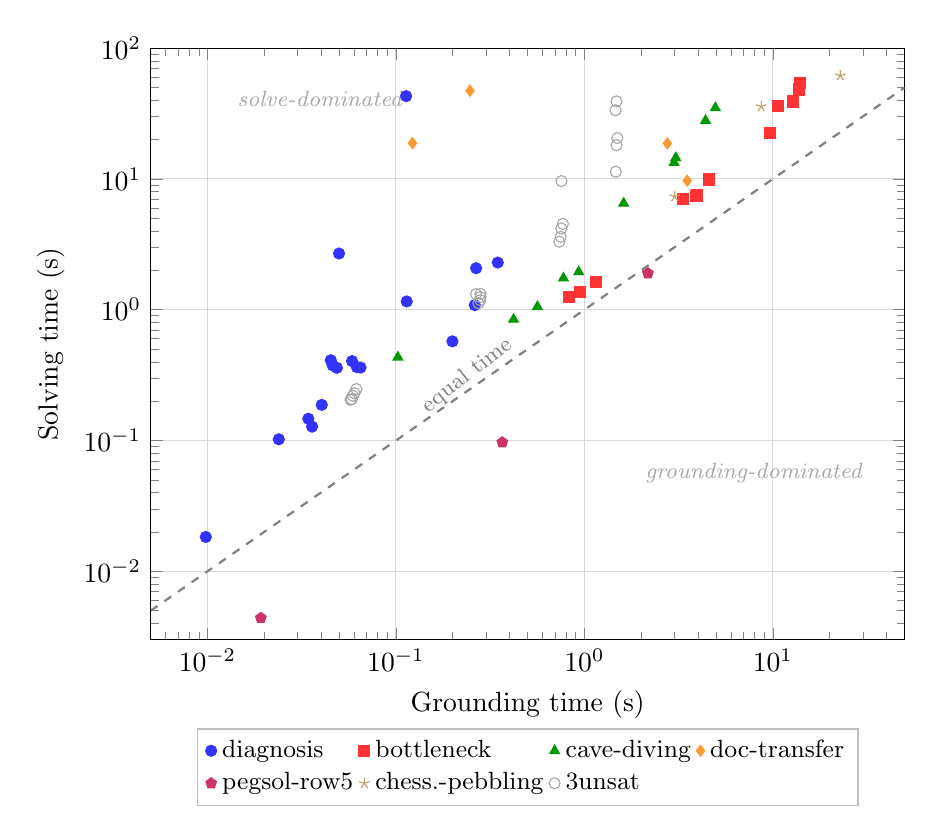
\begin{tikzpicture}
        \begin{axis}[
                xlabel={Grounding time (s)},
                ylabel={Solving time (s)},
                xmode=log,
                ymode=log,
                width=0.92\textwidth,
                height=0.75\textwidth,
                legend columns=4,
                legend style={
                        font=\small,
                        at={(0.5,-0.15)},
                        anchor=north,
                        draw=gray!50,
                        cells={anchor=west},
                    },
                grid=major,
                grid style={gray!30},
                xmin=0.005, xmax=50,
                ymin=0.003, ymax=100,
                mark size=2pt,
            ]
            % y=x reference line
            \addplot[domain=0.005:50, dashed, gray, thick, samples=2, forget plot] {x};
            \node[anchor=south west, font=\footnotesize, gray, rotate=38] at (axis cs:0.15,0.12) {equal time};

            % Solve-dominated region label
            \node[anchor=south, font=\footnotesize, gray!70, rotate=0] at (axis cs:0.04,30) {\textit{solve-dominated}};
            \node[anchor=north, font=\footnotesize, gray!70, rotate=0] at (axis cs:8,0.08) {\textit{grounding-dominated}};

            % diagnosis
            \addplot[only marks, mark=*, color=blue!80] coordinates {
                    (0.0621,0.3639) (0.0649,0.3611) (0.0343,0.1467)
                    (0.2621,1.0846) (0.3471,2.2945) (0.0098,0.0183)
                    (0.0239,0.1022) (0.0359,0.1276) (0.1133,42.9668)
                    (0.0404,0.1873) (0.0499,2.6921) (0.0451,0.411)
                    (0.1994,0.5731) (0.1141,1.1571) (0.0585,0.4049)
                    (0.2664,2.0774) (0.0486,0.3595) (0.0462,0.3755)
                };
            \addlegendentry{diagnosis}
            % bottleneck
            \addplot[only marks, mark=square*, color=red!80] coordinates {
                    (0.8251,1.2573) (0.9501,1.3736) (1.1507,1.6366)
                    (3.3371,7.0537) (3.9382,7.4155) (3.9574,7.5904)
                    (4.6003,9.9099) (9.6922,22.3858) (10.6164,36.0204)
                    (12.7314,39.0981) (13.8004,48.3064) (13.9866,53.7811)
                };
            \addlegendentry{bottleneck}
            % cave-diving
            \addplot[only marks, mark=triangle*, color=green!60!black] coordinates {
                    (0.7743,1.7452) (0.9322,1.9476) (0.5635,1.0549)
                    (0.421,0.8432) (0.1024,0.4335) (4.9541,34.9651)
                    (2.9926,13.3232) (4.3916,27.9326) (3.0535,14.5195)
                    (1.6154,6.5169)
                };
            \addlegendentry{cave-diving}
            % document-transfer
            \addplot[only marks, mark=diamond*, color=orange!80] coordinates {
                    (3.5144,9.7042) (2.7554,18.6905) (0.1224,18.8004)
                    (0.2473,47.2961)
                };
            \addlegendentry{doc-transfer}
            % pegsol-row5
            \addplot[only marks, mark=pentagon*, color=purple!80] coordinates {
                    (0.0192,0.0044) (0.367,0.0968) (2.1726,1.9006)
                };
            \addlegendentry{pegsol-row5}
            % chessboard-pebbling
            \addplot[only marks, mark=star, color=brown!80] coordinates {
                    (3.0178,7.3402) (8.6849,35.7891) (22.7895,61.6811)
                };
            \addlegendentry{chess.-pebbling}
            % 3unsat
            \addplot[only marks, mark=o, color=gray!70] coordinates {
                    (0.059,0.2199) (0.0583,0.2072) (0.0617,0.2474)
                    (0.0574,0.2046) (0.0602,0.2299) (0.2804,1.1825)
                    (0.281,1.3222) (0.2808,1.2488) (0.2661,1.316)
                    (0.274,1.1219) (0.7487,3.6125) (0.7358,3.3119)
                    (0.7542,4.1815) (0.7558,9.6345) (0.7691,4.5319)
                    (1.4634,33.5137) (1.4804,39.1948) (1.481,18.1208)
                    (1.4956,20.5413) (1.4674,11.3587)
                };
            \addlegendentry{3unsat}
        \end{axis}
    \end{tikzpicture}
    \caption{Grounding time vs.\ solving time for all 70 successfully computed instances. The dashed diagonal marks equal time; points above the line are solve-dominated. Only \textit{pegsol-row5} instances fall near or below the diagonal.}
    \label{fig:ground_vs_solve}
\end{figure}
